%\documentclass[a4j,twocolumn,uplatex]{jsarticle}
\documentclass[a4j,twocolumn]{jsarticle}
\usepackage[dvipdfmx]{graphicx}
\usepackage{url}
\usepackage{here}
\usepackage{subfigure}

\setlength{\textheight}{275mm}
\headheight 5mm
\topmargin -30mm
\textwidth 185mm
\oddsidemargin -15mm
\evensidemargin -15mm
\pagestyle{empty}


\begin{document}

\title{Mg-LPSOにおけるL1$_2$クラスターとスモールクラスターの相互作用}
\author{理工学研究科 \hspace{5mm} 情報科学専攻 \hspace{5mm} 47016311 \hspace{5mm} 森下 慎也}
\date{}
\maketitle

\vspace{-1.0\baselineskip}

\section{背景}
我々はMg-LPSO合金におけるLPSO構造の生成機構について,
「積層欠陥部に$L1_2$クラスターが形成され,
そこから排斥されたZn, Yが濃化して新たな積層欠陥を誘発する」という仮説を立てていた\cite{sakamoto}.
これまでの研究では,L1$_2$クラスターと溶質原子単体,あるいはペアとの相互作用を調べるために,L1$_2$クラスターから一層ずつ離れた位置に溶質原子を挿入したモデルのエネルギーを第一原理計算により求めた結果は,
溶質原子がL1$_2$クラスターから離れれば離れるほど安定化するという結果であった.
しかし,この結果に基づいた組織の発展シミュレーションでは,溶質原子の中距離秩序が現れない.


そこで,本研究ではより大きな溶質原子のクラスター集合を仮定し,第一原理計算によりL1$_2$クラスターとの相互作用エネルギーを求めた.

\vspace{-0.2\baselineskip}

\section{手法}
本研究では第一原理計算ソフトVASP(Vienna Ab-initio Simulation Package)を用いて,構造緩和した系全体のエネルギーを求める.
第一原理計算によって,
シュレディンガー方程式を解いて,原子の種類だけから精密
にエネルギーを求め,様々な物性を予測することができる.
VASPは,密度汎関数法による平面波・擬ポテンシャル法を用いた第一原理計算プログラムパッケージである.

平面波基底の第一原理計算では,周期的境界条件が必要となる.
LPSO 構造は積層欠陥が長周期で積層した構造として知られている.
積層欠陥部にはL1$_2$クラスターが存在する.
このクラスターと他の溶質原子の相互作用を求めるためには,
L1$_2$クラスター同士が影響が及ばさないだけの距離をとる必要がある.
本研究では,L1$_2$クラスター同士が20 層離れている,24層のslab モデルを用いる.


\section{スモールクラスターについて}
清原らはhcp構造にL1$_2$クラスターを導入すると,
構造緩和により2つに分割されたスモールクラスターが生成されると報告していた\cite{kiyohara}.
しかし,L1$_2$クラスターがどのように分割されるかは報告されていなかった.

そこで,図\ref{fig:three}の(a),(b)のように,
L1$_2$クラスターを上下,左右方向に分割したスモールクラスターを,
hcp-Mg結晶に挿入したモデルについて第一原理計算をおこなった.
計算結果は上下方向に分割した(a)のエネルギーが0.2eV程度低く,
(a)の方がMg結晶内においてより安定する事を示している.
よって,(a)をスモールクラスターとして計算をおこなった.

図\ref{fig:one}に示すスラブモデルにスモールクラスターを挿入し系全体のエネルギーを求めた.
図\ref{fig:one}において同じ色で示した等価な位置へスモールクラスターを配置したモデルについて第一原理計算をおこなった.

\begin{figure}[H]
\vspace{-1.3\baselineskip}
\begin{center}
   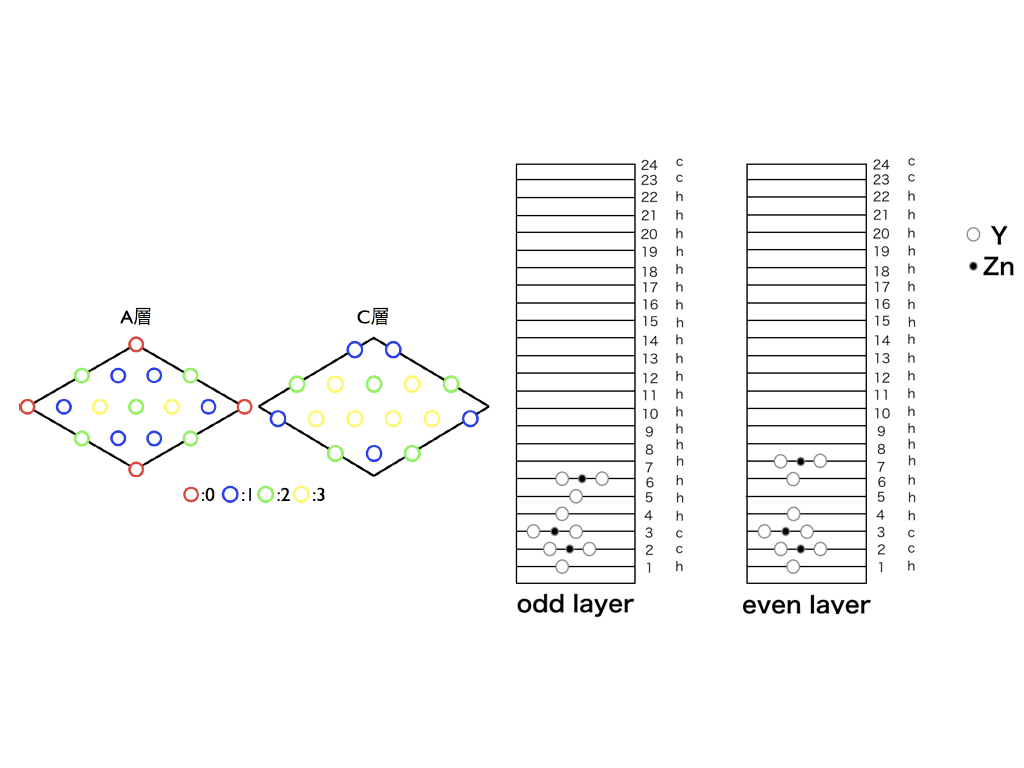
\includegraphics[width=80mm]{./slab24_color.jpeg}
   \vspace{-0.6\baselineskip}
  \caption{A 層とC 層における近接距離を表した図と計算に使用する24層モデルの模式図.}
  \label{fig:one}
\end{center}
\end{figure}

\begin{figure}[h]
\vspace{-2.0\baselineskip}
\begin{center}
   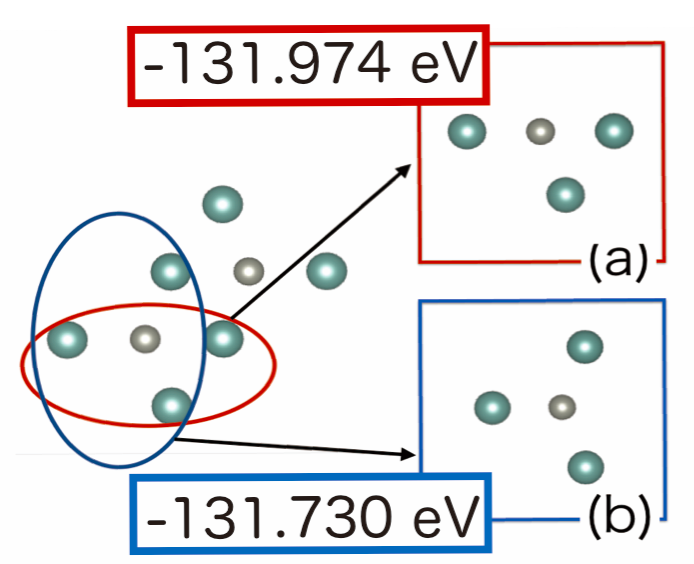
\includegraphics[width=60mm]{./dividing_cluster.png}
  \caption{L1$_2$クラスターの分割方法を示している.(a),(b)はそれぞれL1$_2$クラスターを上下,左右方向に分割したモデルを示している.}
  \label{fig:two}
\end{center}
\end{figure}
\vspace{-2.0\baselineskip}

\section{L1$_2$クラスターとスモールクラスターの相互作用}

図\ref{fig:three}にL1$_2$クラスターとスモールクラスター間の垂直距離による系全体のエネルギーの変化を示した.
エネルギー値は4-5層離れた位置で最低値となり,
6層以上の距離でも単調に減少することはなかった.
これは4-8層で見られるエネルギーの上昇が周期的に並ぶ他のL1$_2$クラスターの影響によるものでない事を示唆しており,
僅かではあるが中距離で溶質原子が安定する傾向を示している.

\begin{figure}[H]
%\vspace{0\baselineskip}
\begin{center}
   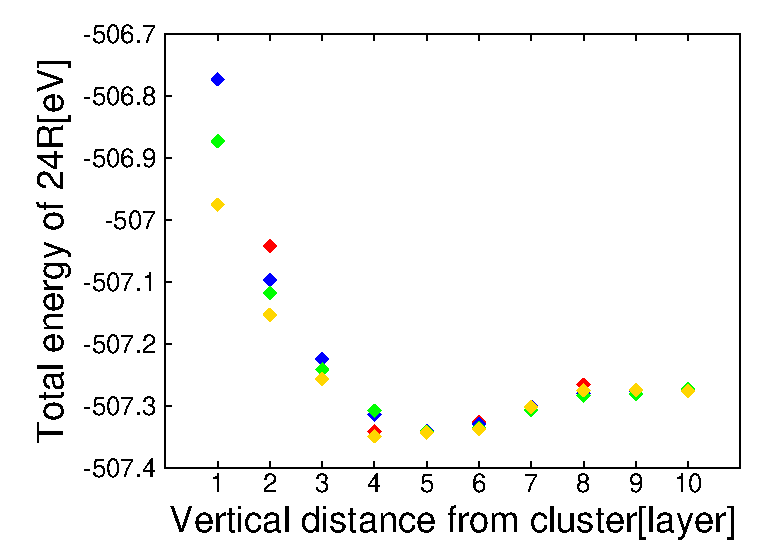
\includegraphics[width=80mm]{./smallcluster_Alld_JPS2017.eps}
  \caption{L1$2$ クラスターとスモールクラスターの距離によるエネルギー変化.グラフの点の色は図1で示した近接距離の色に対応している.}
  \label{fig:three}
\end{center}
\end{figure}

\vspace{-1.0\baselineskip}

\section{スモールクラスターの拡散法について}
エネルギー的に得られた中距離での安定性から,
動的な組織形成機構を解明するためには,
スモールクラスターの拡散機構について議論をおこなう必要がある.
拡散法として,単空孔を利用した空孔拡散,
あるいは複空孔を利用したクラスター拡散をおこなうという予想を立てた.

原子の拡散法として広く知られている空孔拡散は,
図\ref{fig:four}(a)に示すように,
原子の存在しない格子点と原子が位置を入れ替えることで起きる拡散である.
それに対し,今回それに加えて予測しているクラスター拡散は,
図\ref{fig:four}(b)に示すように,
複空孔とそれに対応した原子数のクラスター集団が位置を入れ替えるものを考えている.
空孔拡散はactivation barrierを超える必要があるため,
クラスター拡散の方が拡散の可能性は高くなり,
より早く拡散される.

両方の拡散法において,
空孔を利用するということが共通する事項として考えられる.
よって,空孔がスモールクラスターの近くで安定するかを第一原理計算によって確かめる.

\begin{figure}[htbp]
\begin{center}
    \subfigure[空孔拡散の模式図.]{%
        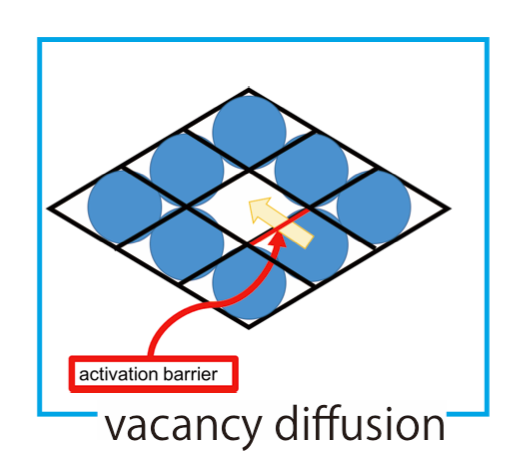
\includegraphics[clip, width=0.4\columnwidth]{./vacancy_diffusion.png}}%
    \subfigure[クラスター拡散の模式図.]{%
        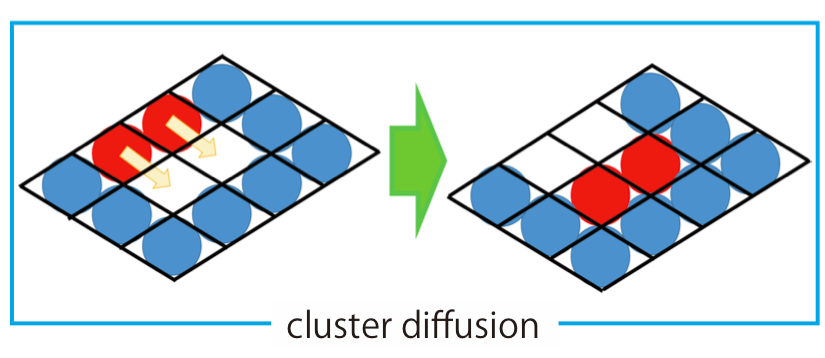
\includegraphics[clip, width=0.5\columnwidth]{./cluster_diffusion.png}}%
    \caption{拡散法の模式図.}
    \label{fig:four}
\end{center}
\end{figure}

\vspace{-1.0\baselineskip}

\section{スモールクラスター付近での空孔の安定性}

まず,単空孔を用いた空孔拡散,あるいはクラスター拡散がおこなわれる可能性を確かめるためにスモールクラスターの周辺に空孔を挿入したモデルを作成した.

図\ref{fig:five}に単空孔を挿入したモデルと第一原理計算により求まった計算結果を示す.
単空孔を用いた拡散がおこなわれるとすれば,
図\ref{fig:five}中の(b)の位置で単空孔が安定することになる.
しかし,その予想に反して,
計算結果は一番離れた位置である(c)の位置で単空孔が安定する事を示唆した.

図\ref{fig:six}はスモールクラスターの上部に2層ずつ離して隣接した空孔を挿入したモデルと,スモールクラスターと複空孔の距離によるエネルギー変化を示したグラフである.
計算結果は5層離れた位置で再安定値をとっており,こちらもスモールクラスターの近くで安定するという仮説を支持しなかった.


\begin{figure}[H]
%\vspace{0\baselineskip}
\begin{center}
   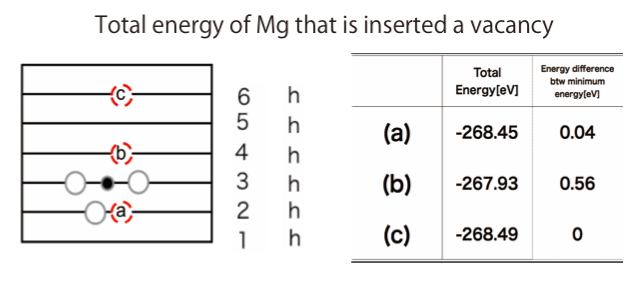
\includegraphics[width=80mm]{./vacancy.png}
  \caption{スモールクラスター周辺に単空孔を挿入したモデルと,系全体のエネルギーをまとめた表.}
  \label{fig:five}
\end{center}
\end{figure}

\begin{figure}[H]
\vspace{-1.0\baselineskip}
\begin{center}
   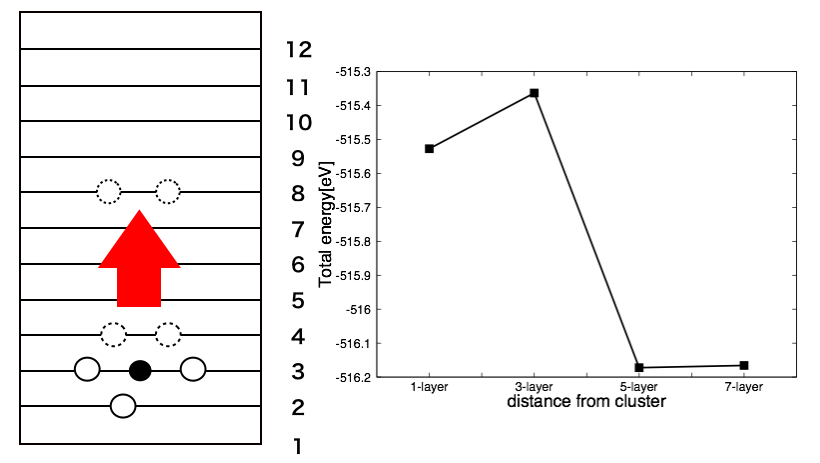
\includegraphics[width=80mm]{./double_vacancy.png}
  \caption{スモールクラスター上部に複空孔を挿入したモデルと,スモールクラスターの距離によるエネルギー変化を示すグラフ.}
  \label{fig:six}
\end{center}
\end{figure}

\vspace{-1.4\baselineskip}

\section{まとめと今後の課題}
第一原理計算の結果から,
溶質原子はスモールクラスター単位で積層欠陥から中距離で安定するということが示された.
よって,当初立てていたシナリオは,
「積層欠陥部に$L1_2$クラスターが形成され,
そこから排斥されたZn, Yが,スモールクラスターを形成することで濃化し,
新たな積層欠陥を誘発する」というシナリオに修正された.

しかし,拡散法として考えていた空孔拡散,あるいはクラスター拡散については,
スモールクラスター付近での空孔の安定を支持する結果は得られず,
溶質原子がどのように拡散するかは特定できていない.

スモールクラスターを挿入した計算結果は中周期安定を示したが,過去の計算に比べて大きなモデルを使用したことも要因として考えられるため,今回の結果を踏まえてさらなる追求をが必要となる.加えて,拡散法についてもさらなる検証をおこなうことが今後の課題となる.
\vspace{0.2\baselineskip}

{\small\setlength\baselineskip{10pt}	% 参考文献は小さめの文字で行間を詰めてある
\begin{thebibliography}{9}
\bibitem{sakamoto}Y. Sakamoto, C. Shirayama, Y. Yamamoto, R. Kubo, M. Kiyohara, and S. R. Nishitani: Mater.Trans., 56(2015), 933.
\bibitem{kiyohara} M. Kiyohara, et al., proceedings of PRICM, (Kyoto 2016).
%\bibitem{okuda}H. Okuda, M. Yamasaki, Y. Kawamura, M. Tabuchi, H. Kimizuka: Scientific Reports 5 (2015), 14186.
\end{thebibliography}
}

\end{document}
